\documentclass{article}
\usepackage{graphicx}


\begin{document}

\title{CMSC 471: Project 3}
\author{Lee Brown}

\maketitle

\begin{figure}[h!]
  \centering
  
\includegraphics[scale=.5]{11.jpg}
  \caption{A sample image.}
\end{figure}

\section{Introduction}
The purpose of this project was to use a support vector machine to make a basic image recognition software. The packages, language, and versions used for this project are as follows:

\begin{itemize}
\item Python 3.5.1
\item Anaconda 2.5.0 
\item numpy 1.10.4
\item sklearn 0.17
\item Python Image Library
\end{itemize}

\section{Method}

\begin{figure}[h!]
  \centering
  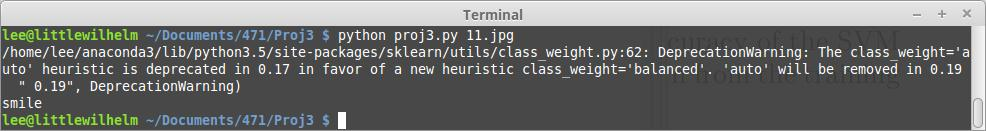
\includegraphics[scale=.40]{prediction.jpg}
  \caption{The program predicting the above smiley face.}
\end{figure}

The process used for this project is a multi-step process. The first step is loading and processing the training set. The program opens the location of the training set and processes the files one by one. By using the Python Imaging Library’s (PIL) functions for images and list comprehensions, it was easy to make the transition from an image to the image’s normalized bitmap. The steps for completely processing the image were

\begin{itemize}
\item Open the image.
\item Get the list of tuples containing the pixel data using PIL’s getdata().
\item Flatten the list of tuples into just a 1-dimensional list of integers.
\item Normalize the list by dividing each entry by 255.
\end{itemize}

The normalized list of pixel values were stored in the main function in a large, 2-dimensional list named tempList. Alongside of that list, the items were also being classified by storing a value in another list called classifierList, that saved a string describing the image based on which directory it was opened from.



Once all of the images were processed, the Sci-kit Learn SVM was created. By using the class weight setting of “auto”, I increased the accuracy of the SVM significantly. The two lists are passed in together for it to learn from the training set, and prepare it for the test. 

The test image is then loaded and processed like the training images, and the SVM is used to predict what type of image it was. It then prints out the results.


\end{document}
